\subsection{Electromagnetic Calorimeter} 
\label{sec:ecal}

The Ecal, depicted in Figure \ref{fig:ecal}, consists of $442$ lead-tungstate PbWO$_4$ crystals with avalanche photodiode (APD) 
readout and amplifiers. The short output pulse widths permit operation at very high rates. Indeed,(PbWO$_4$) crystals with APD readout 
are ideally suited to deal with the expected high radiation and high rate environment and they can operate in the fringe field of the HPS
magnetic field as well. The lead-tungstate modules, see Figure \ref{fig:module}, are taken from the Inner 
Calorimeter (IC) of the JLab CLAS detector, which was built by IPN Orsay (France) and other Hall B collaborators and was used
in a series of high energy electroproduction experiments. 
Orsay played a key role in the design and fabrication of the support frames, thermal enclosure, amplifiers,  
and motherboards of the IC, and is playing a similar role with the HPS ECal.  
The PbWO$_4$ crystals are $16$ cm long and tapered. The cross section of the front face is $1.3\times 1.3$ cm$^2$, 
and  $1.6\times 1.6$ cm$^2$ at the back. Modules in the ECal are arranged in two formations, as shown in Figure \ref{fig:ecal}. 
There are 5 layers in each formation; four layers have $46$ crystals and one has $37$. The ECal is mounted downstream of the 
analyzing dipole magnet at the distance of about $137$ cm from the upstream edge of the magnet. The two ECal modules are 
positioned just above and below the ECal vacuum chamber, through which the beam, radiated photons, and the wall of flame will pass
unimpeded. The innermost edge of the crystals is just $2$ cm from the beam. In order to stabilize the calorimeter's performance, 
the crystals, APDs, and amplifiers are enclosed within a temperature controlled environment, held constant at 
the level of 1\!\char23F. The energy resolution of the system, expected from operational experience with the IC, 
is $\sigma_E/E \sim 4.5\%/\sqrt{E}$ (GeV). As in the IC, PbWO$_4$ modules are connected to a motherboard that provides
power and transmits signals from individual APDs and amplifier boards to the data acquisition system. The ECal data is 
digitized using the JLAB FADC250, a 250 MHz flash ADC developed for the 12 GeV Upgrade. Pulse height information and spatial 
and timing information from each crystal are available for the trigger decision, which uses this information to reduce the trigger rate to a manageable $\sim 30$ kHz (see Section \ref{sec:triggerdaq} 
for details).

\begin{figure*}[t]
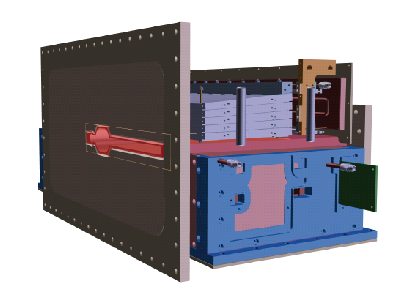
\includegraphics[width=\textwidth]{ecal/ECal.png}
\caption{\small{Arrangement of Ecal crystals. The two modules are positioned above and below the beam plane. Each module has 5 layers. 
There are 46 crystals in each layer, with the exception of the layers closest to the beam plane in which 9 crystals are removed to allow 
a larger opening for the outgoing electron and photon beams.}}\label{fig:ecal}
\end{figure*}

\begin{figure*}[t]
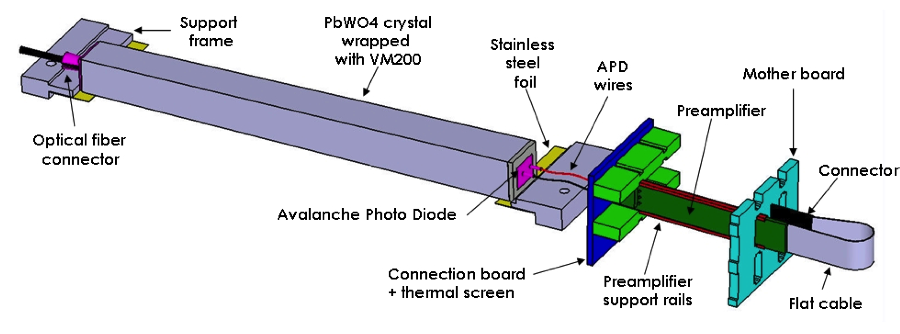
\includegraphics[width=\textwidth]{ecal/ecal_module.png}
\caption{\small{The ECal module is composed of a 16 cm long lead-tungstate crystal, Avalanche Photo Diode, and a amplifier 
board.}}\label{fig:module}
\end{figure*}

The HPS calorimeter described above was built and used during the HPS test run in April-May of 2012. This was the first time that 
a readout and trigger system utilizing the JLAB FADC250s had been used in a real experiment. The trigger algorithm was designed 
to satisfy the HPS 
event selection criteria and was implemented with newly developed FPGA-based trigger processors. Not all aspects 
of the trigger system were tested in the HPS Test Run because of the low interaction and background rates associated with photon running. But the 
ECal and its readout performed well and the critical goals for the Test Run run were 
achieved (see Section \ref{sec:testrun2012} for details). While the ECal performance during the test run was satisfactory, several aspects are in need of improvement, as described below.   

\subsubsection{Improvements to the existing calorimeter}

There are no plans for major mechanical changes to the ECal proper. The crystals, support frames, and thermal enclosure operated as designed and will stay unchanged. Most of the needed changes are related to the signal readout chain and problems encountered in the Test Run with the ECal and FADC250. Plans for  
modifications and/or improvements are as follows: 

\begin{enumerate}
\item {\bf Replacing the ECal mounting system} - 
During the test run the ECal was supported by the Hall-B pair spectrometer mount rails which also support with the pair spectrometer hodoscopes. 
Photon running prevented the installation of the ECal vacuum chamber and relaxed the requirements for precise ECal alignment. Consequently, the ECal was simply hung from the mount rails using  long threaded rods. This system must be replaced with a more robust and finely adjustable (both horizontally and vertically) support mechanism to  align the  ECal correctly with the ECal vacuum chamber.

\item {\bf Modifications to the side brackets to accommodate fiber bundles for the light monitoring system} -
A light monitoring system was not used during the test run. While the design of the ECal enclosure was done in such a way that it can 
accommodate optical fibers attached to the front face of crystals, the side plates that hold the crystal frames do not have inlets for the accompanying fiber bundles.
Space is available on the side plates for a straight-forward modification which will allow the addition of a light monitoring system.  
    
\item {\bf Modification of motherboards} - One of the issues  faced during the test run was excess noise on some channels of the motherboards. 
Most missing channels, those which are absent on the performance figures in Section \ref{sec:testrun2012}, were in fact switched off because they were very noisy and there was no time to debug them. New motherboards will be designed and built to resolve these noise issues. One of options under discussion is to replace long motherboards with shorter ones with power and signal connectors 
located on the top (for the top module) and the bottom (for the bottom module) of the thermal enclosure. 

\item {\bf Signal splitting} - From the experience gained with the JLAB FADC250 by the HPS group and others, it is evident that the FADCs can be used both for precision time measurements and as 
real-time scalers simply by developing the appropriate firmware.
Precise pulse timing will allow tighter coincidence windows and lower backgrounds, and real time scalers will provide good online monitoring of detector performance. The present ECal readout configuration uses signal splitters to divide the preamplifier signal in  a 2:1 ratio, sending 
$2/3$ of the signal to a discriminator that has built-in scalers and feeds the TDC channel. The other $1/3$ of the 
signal goes to the FADC for the energy measurement. Removing the splitter will increase the signal on the FADC input by $\times 3$. This will allow lowering the amplifier gain and thereby lowering the noise level. This effort will make use of developments already planned for other detectors at JLAB.

 
\item {\bf New preamplifiers} - The noise will be further reduced with the addition of new preamplifiers, allowing an additional reduction in effective energy threshold. The impact of the lower noise/threshold system is twofold: first it 
will improve the ECal's energy resolution; and second it will make the ECal sensitive to minimum ionizing particles which pass through the crystals transversely. With sensitivity to cosmic ray muons, which will pass through the ECal transversely when it is installed in HPS, the Ecal crystals can be calibrated for MIPS, and their effective gains balanced.  HPS collaborators from INFN Genova have shown that with such a low noise, low threshold system, the ECal can distinguish the MIP energy deposition from noise, see Figure \ref{fig:mip10x10}and explanations below.

\item {\bf Light monitoring system}

For an experiment like HPS, where backgrounds must be well understood and need to be strongly suppressed, the trigger bias must be minimized. In particular, having stable, known, and uniform thresholds at the trigger readout is necessary in order to avoid  bias in the 
event selection. Such uniformity and stability can be achieved with the installation of an online gain monitoring 
system. This system will introduce short light pulses into the front face of the crystals. The crystals already have fiber holders attached, allowing implementation of this system without having to modify the crystals or wrapping. 

Optical fibers will be used to transmit light from a calibration  source to the crystals to test the response of the APDs. The response of the system could change in time because of 
losses in crystal transparency due to radiation damage or because of gain variations of the APDs. 
Such a calibration system has been developed for several experiments (CMS at CERN for instance) with various light sources. The system for the ECal 
will be developed at IPN Orsay during 2013 and in the first half of 2014, and will be ready for installation at JLAB for the commissioning run in the fall of 2014. Each module will have a red and blue mono-color LED light source for monitoring purposes. 
Blue light transmission, corresponding to the domain of the crystal's emission spectrum, is very sensitive to the presence of color centers which are produced by radiation damage. So the blue light source will monitor variations of the response in the main domain of the spectrum.
 %Impurities can anneal at room temperature and such monitoring can be sensitive to increasing of output as well, when the radiation exposure is reduced for a long period of time. 
The response to red light is less sensitive to the color centers,  and so permits monitoring the APD gains more directly. Thus the use of two colors separates gain variations due to the 
APD and electronics from those due to changes in the crystal transparency, and provides clear information on the state of the electronics. 
The main challenge for the system is to guarantee stability at a level of $2\%$. The test of the system will be carried-out at
IPN Orsay, in order to study its efficacy and also to test the radiation resistance of the various materials.

\item {\bf New low-voltage power supply} - The existing low voltage power supply is a manually controlled, single output power supply 
that feeds the four ECal motherboards through a custom-made patch panel. The present system cannot control the voltage supplied to preamplifiers at different
parts of the ECal, and controlling or resetting them remotely has proved to be very inconvenient, requiring frequent access to the Hall, especially during commissioning. Newly available low voltage power supplies are much more flexible. The one that is the most suitable for the
ECal APD preamplifiers is the WIENER MPV 8008LD. This power supply is being used at JLAB and the control software exists, so it will be easy to incorporate it into HPS.     

\end{enumerate}
  

\subsubsection{Possibilities with new APDs} 

Installing new APDs on the current crystals will significantly improve the ECal performance, but doing so is expensive,  so replacement is only being considered if a funding source beyond DOE HEP is secured. Replacing the old $5\times 5$ mm$^2$ 
Hamamatsu S8664-55 APDs with $10\times 10$ mm$^2$, Hamamatsu S8664-1010 will improve two critical characteristics of the present calorimeter modules. First, the new APDs from Hamamatsu have much better performance than the ones which are currently installed. Data from Hamamatsu shows that APDs made from the same wafer have excellent gain uniformity. With $\pm 10\%$ known uniformity 
at the gain of $100$, the required variations in bias voltage are only $\sim 4.5$ V. Even for large samples of APDs (~1300),  the required bias voltage differences are ~50 V, which is half that of the current APDS. The ECal supplies bias voltage to groups of APDs, so with new APDs, with their smaller voltage-gain variations, it will be possible to achieve much better 
uniformity in the response of the calorimeter modules, and consequently better uniformity in trigger thresholds. 

Secondly, the new APDs have a $4$ times larger readout area, ensuring $4$ times more light collection and therefore $4$ times larger signals. This will allow the use of lower gain amplifier modules which in turn will decrease electronic noise. Tests 
performed for another calorimeter, now in production at INFN Genova for JLAB Hall-B, showed that amplifier boards 
with a factor 2 lower gains have a noise level $<5$ MeV. The energy deposition in the HPS PbWO$_4$ crystals  
from minimum ionizing cosmic muons passing transversely to the crystal axis is $\sim 15$ MeV. Moving the energy thresholds 
close to $5$ MeV will allow the MIP peak to be clearly distinguished, and will let the calorimeter  be calibrated and monitored with cosmic muons. The HPS collaborators 
from the INFN group have performed the first tests of the Hamamtsu $10\times 10$ mm$^2$ APDs and a new amplifier board on HPS crystals. In 
Figure \ref{fig:mip10x10}, the charge distribution of a single crystal system is shown for $5\times 5$ mm$^2$ (left) and $10\times 
10$ mm$^2$ (right) APDs. A coincidence signal from scintillator telescopes positioned above and below the module provides the trigger. 
The crystal was positioned horizontally as it would be in HPS, so the cosmic muons would pass through it perpendicular to the crystal axis. The red line 
histogram is for all events triggered by the scintillation telescope and corresponds to the noise. The black line histogram corresponds 
to the charge detected within $100$ ns of the trigger time. The MIP peak is clearly visible and well isolated from the noise 
for the S8664-1010 APD readout. For  the S8664-55 APD, the MIP signal is also seen, but its charge distribution is under the noise peak and it
does not have well defined peak position. Using MIP calibration in conjunction with the light monitoring system will ensure stable and reliable performance of the ECal and the trigger system. As a bonus, the lower noise will allow the use of lower  thresholds and improve the calorimeter's energy resolution. The new amplifier boards have to be designed to work with new APDs. 

\begin{figure*}[t]
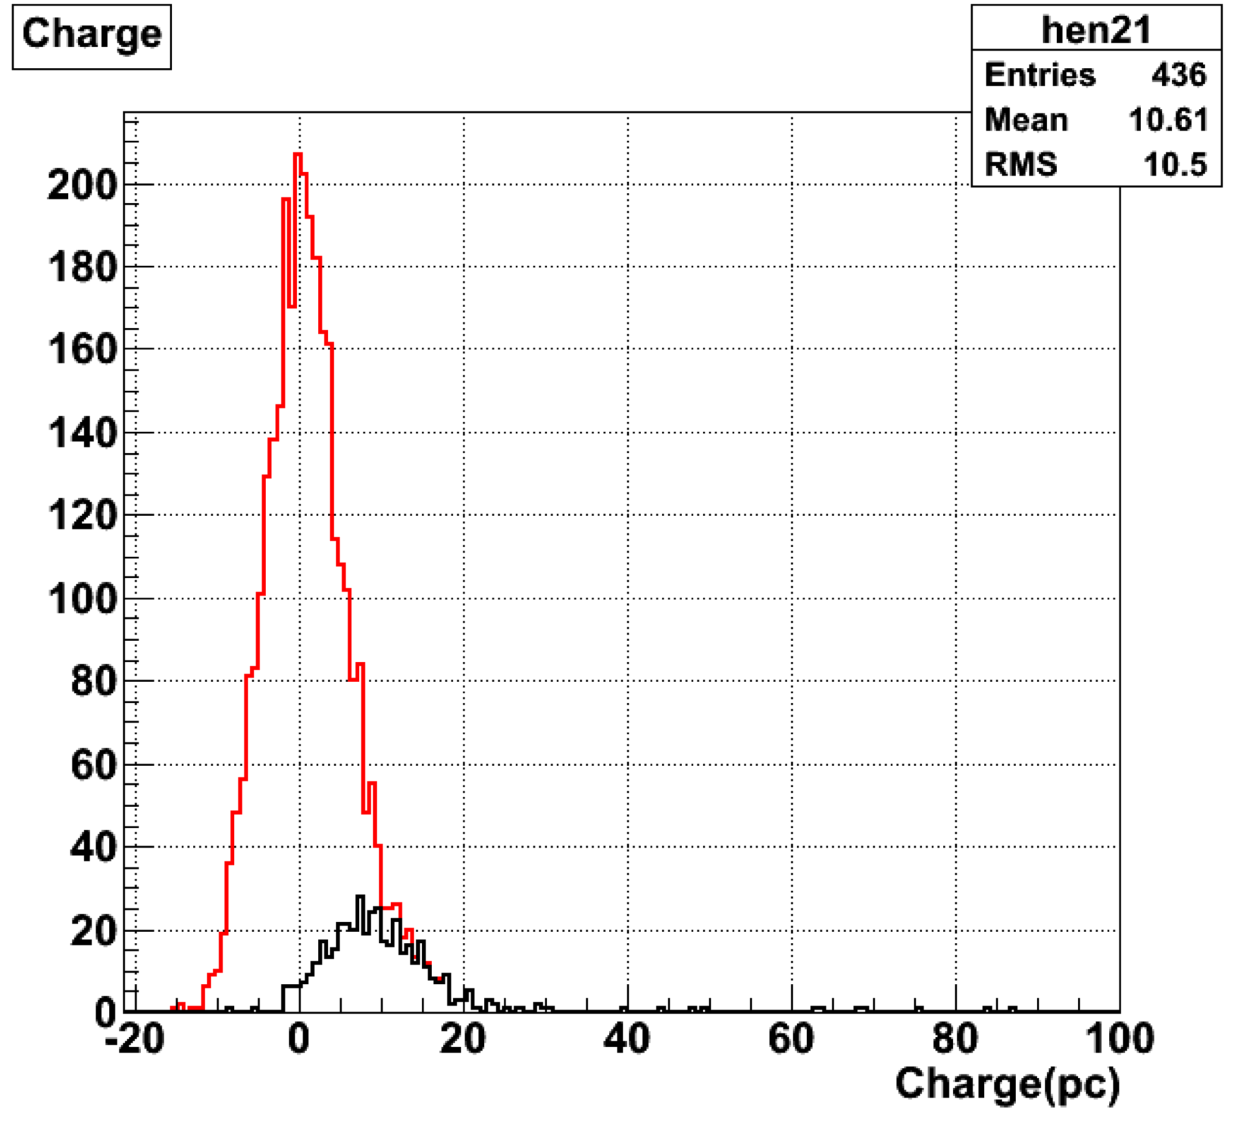
\includegraphics[scale=0.37]{ecal/MIP_5x5_APD.png}
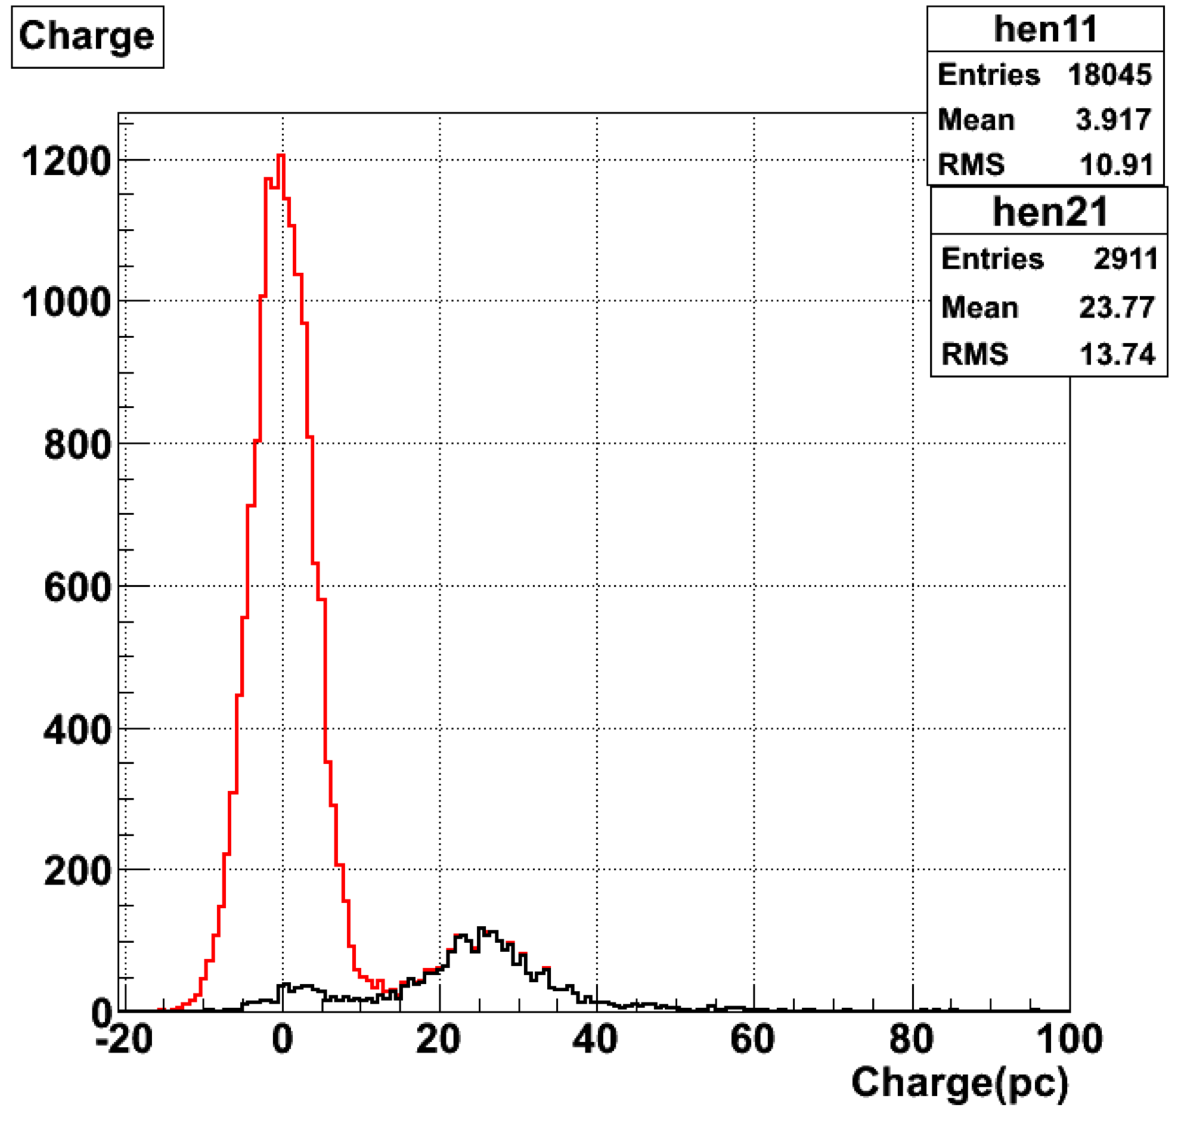
\includegraphics[scale=0.37]{ecal/MIP_10x10_APD.png}
\caption{\small{Charge distribution from readout of the HPS calorimeter crystal with Hamamatsu S8664-55 (left) and S8664-1010 
(right) APDs, and the new low noise amplifier board. The red line histogram corresponds to the charge distribution for all triggers 
comming from the scintillators positioned above and below the crystal. The black line shows the distribution for hits in the crystal 
within $100$ ns of the trigger signal. }}\label{fig:mip10x10}
\end{figure*}

The total cost of replacing all ECal APDs is about $500$K\$. The HPS collaborators from IPN Orsay have applied for a  
European Research Council (ERC) Advanced Grant 2013 to purchase APDs, for manpower costs to replace the old ones, to design and build 
new preamplifier boards, and to assemble and test the ECal with the new modules. This grant also includes light monitoring system. If successful the grant will cover most of the ECal modifications, and will significantly reduce the support needed from DOE for the more modest upgrades we have proposed above. 
